\documentclass{article}

\usepackage{graphicx}
\usepackage{epstopdf}
\usepackage{caption}
\usepackage[section]{placeins}


\title{  Exercise 3 \\
        \large Deep Learning lab}
%\author{Silvio Galesso}
\date{}

\begin{document}
\maketitle

\section*{Scenario 1}
	\begin{figure}[!htb]
        \centering
        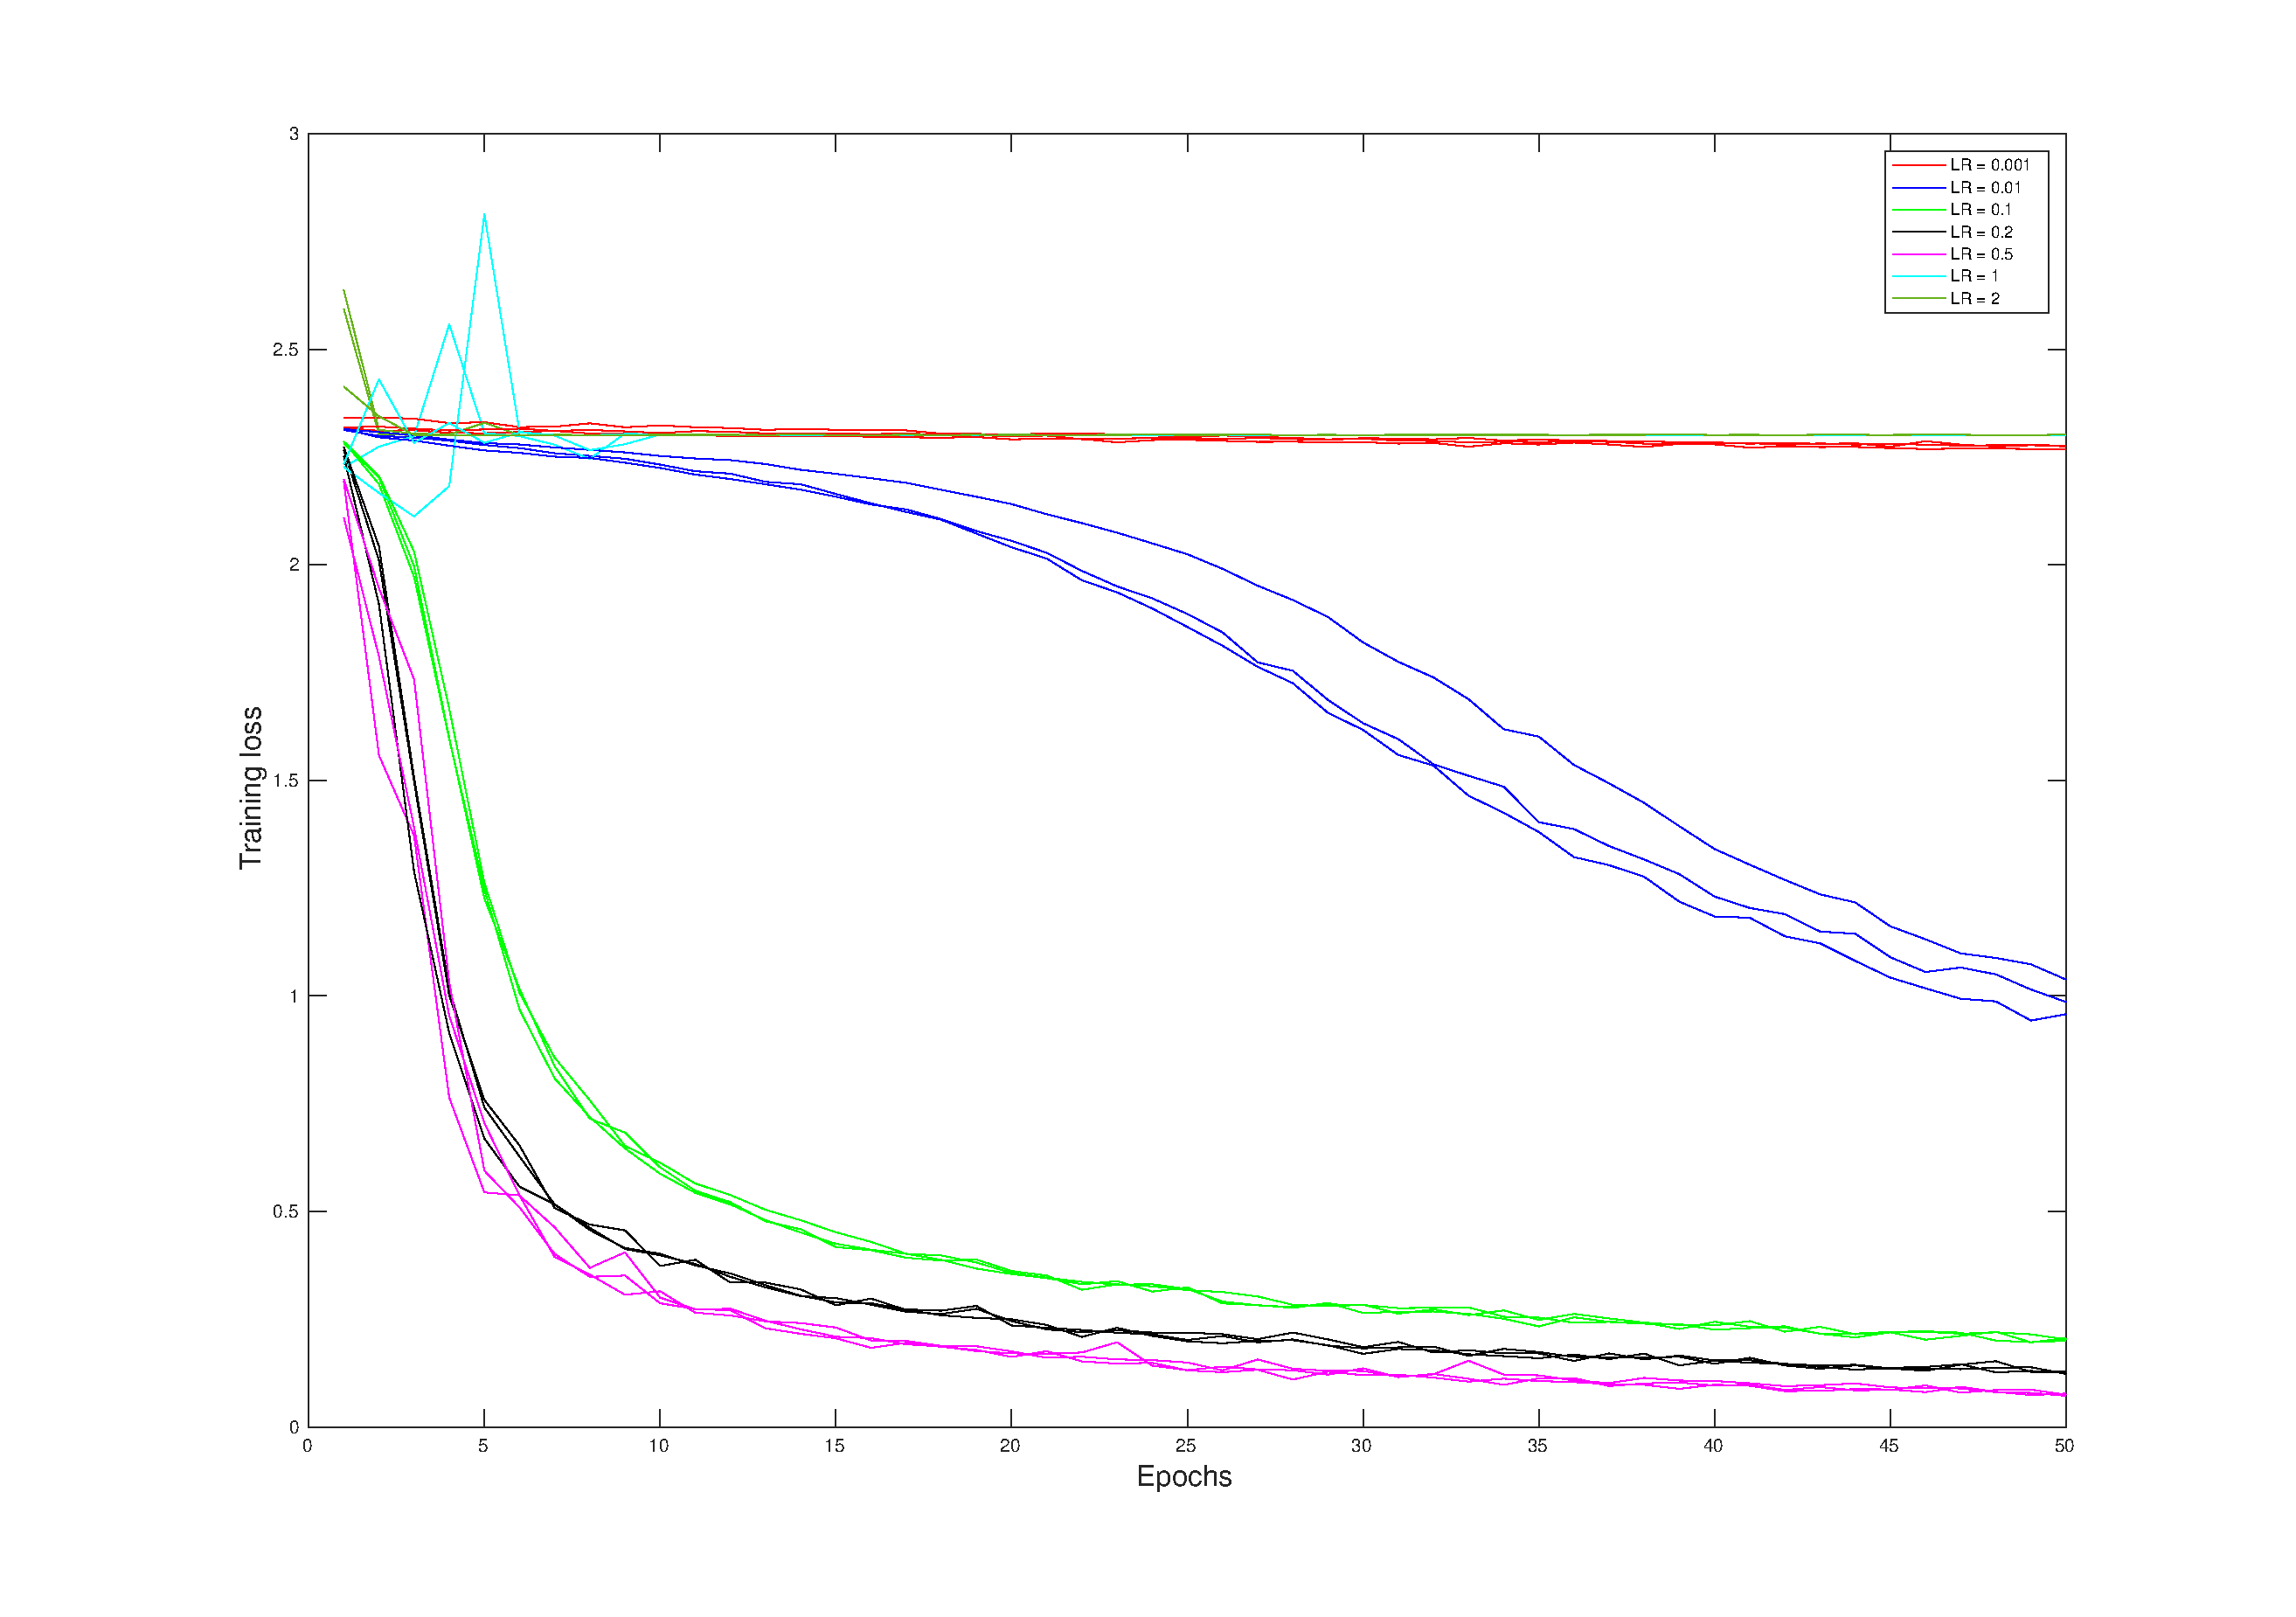
\includegraphics[width=\textwidth]{figures/sc1_tr_loss}
        \captionsetup{labelformat=empty}
        \caption{Figure 1.1}
    \end{figure}
    \begin{figure}[!htb]
        \centering
        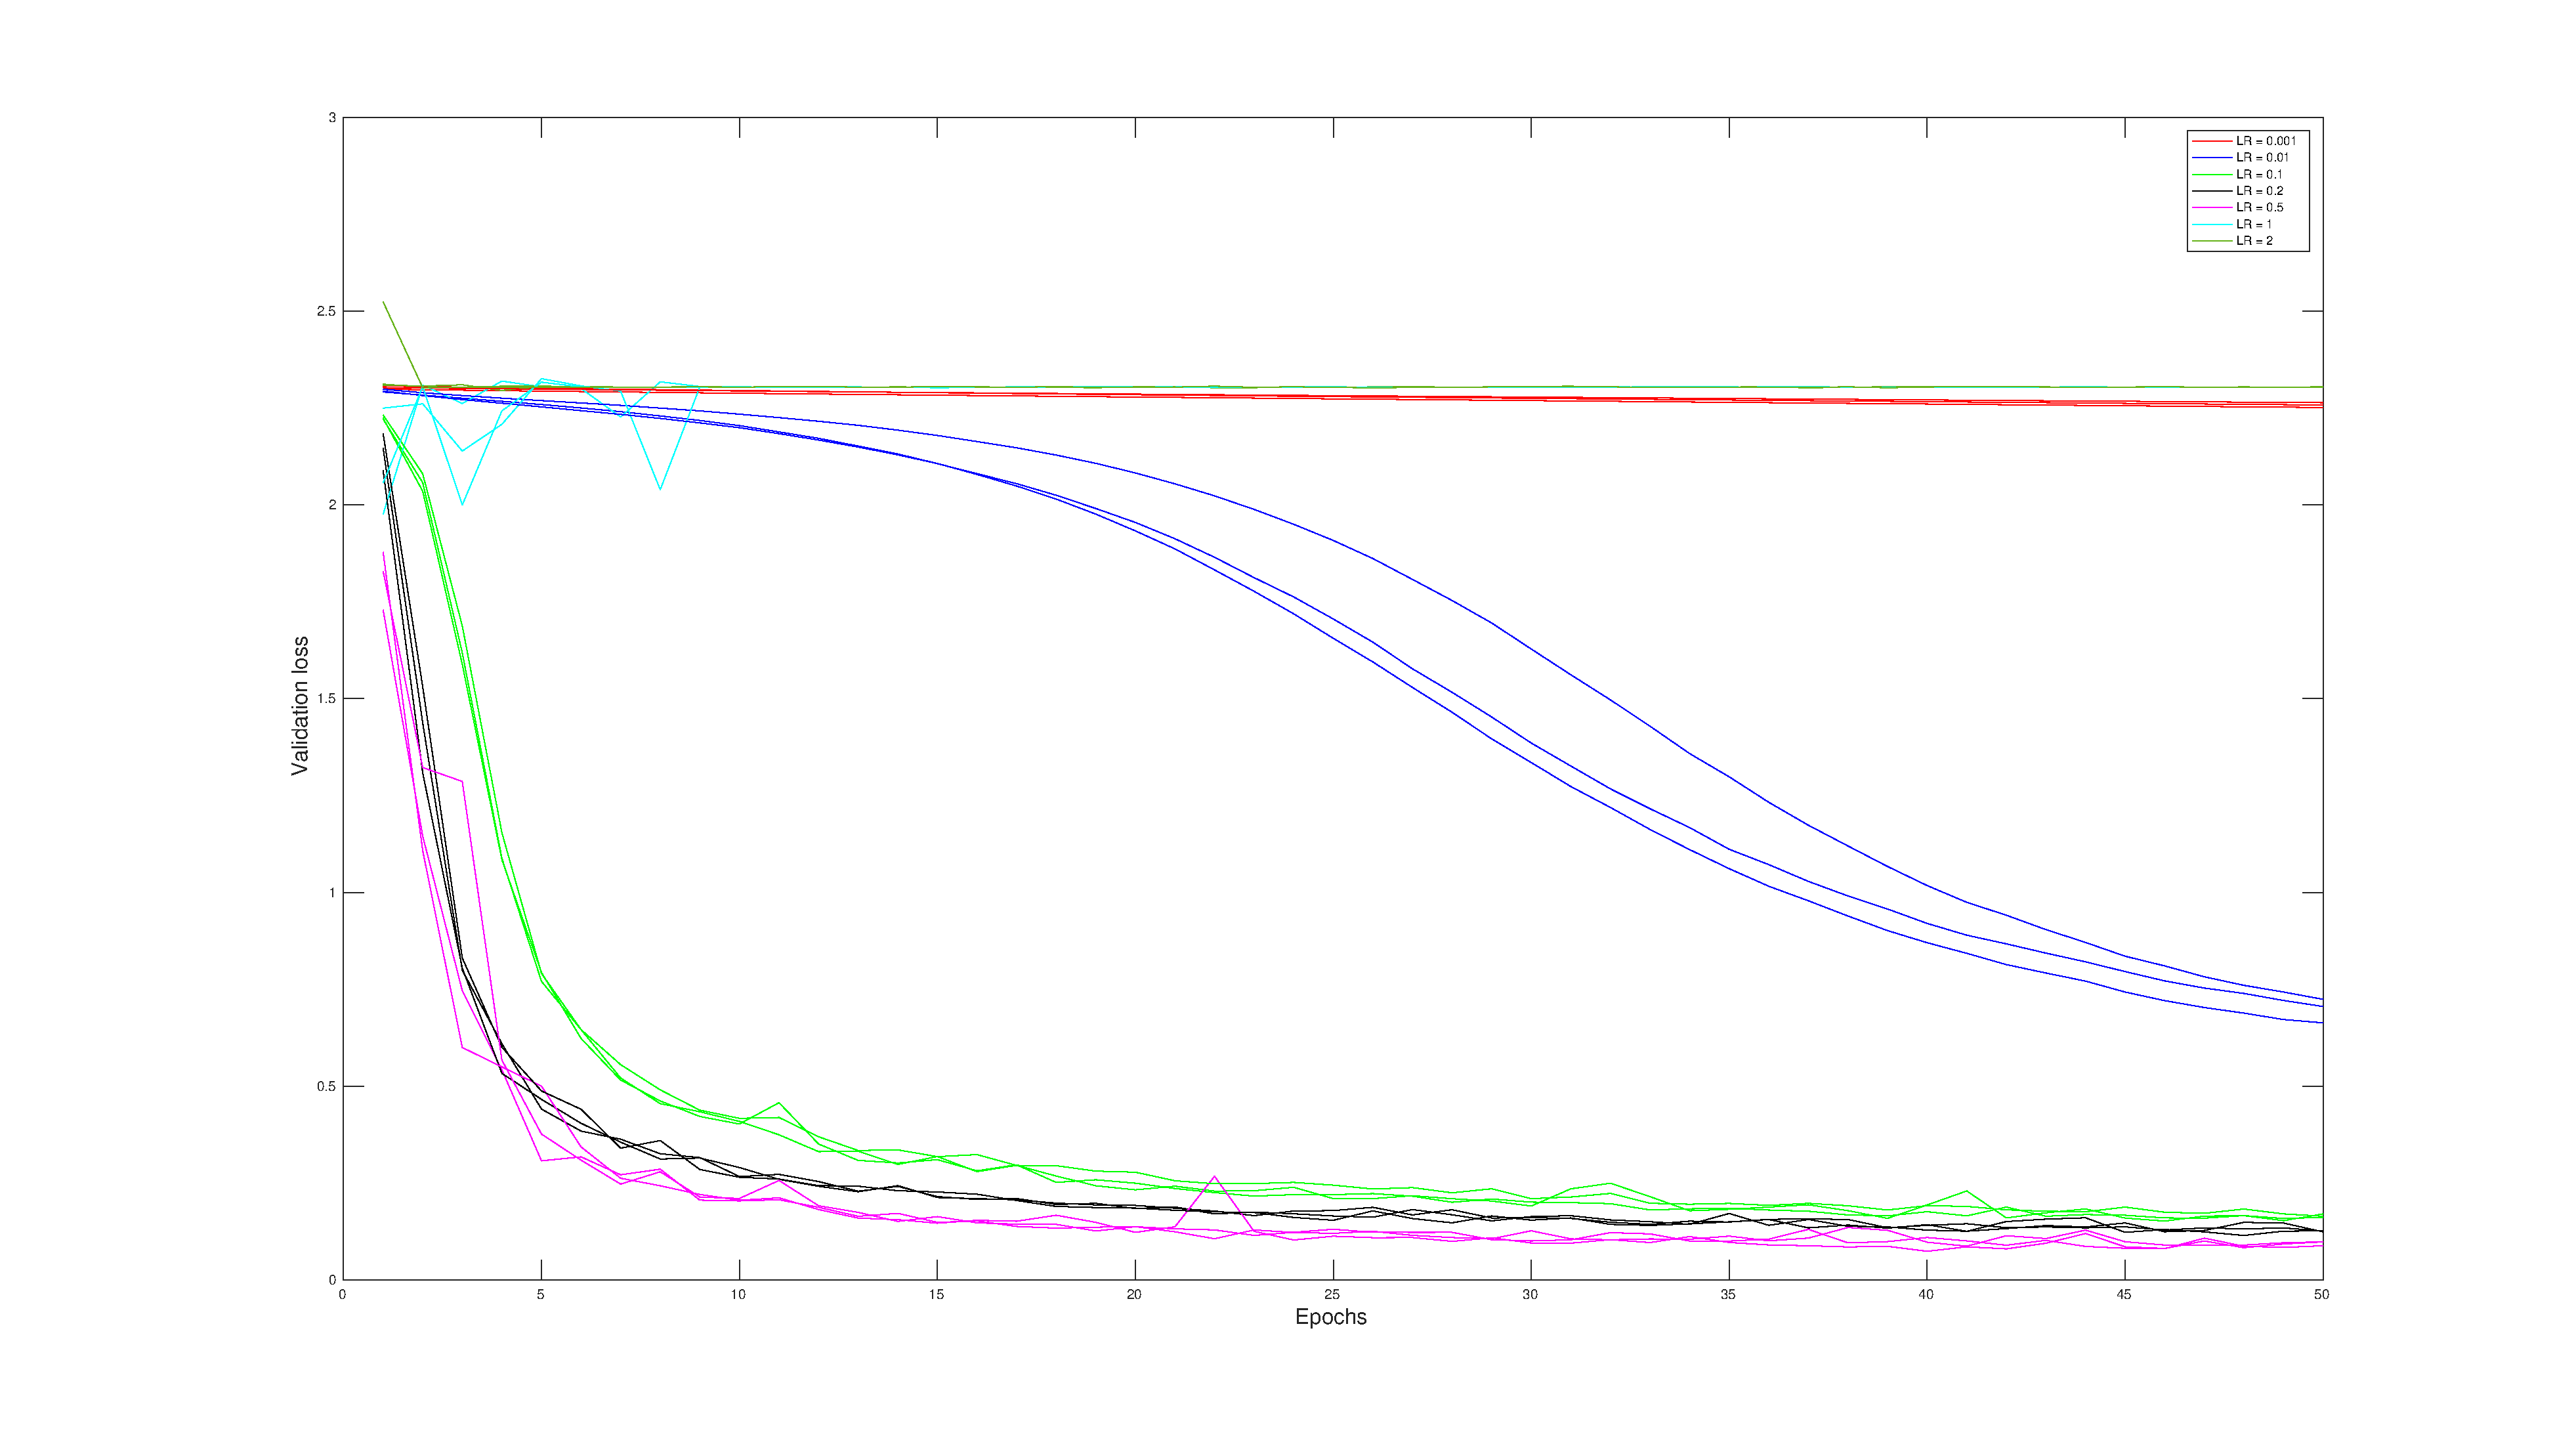
\includegraphics[width=\textwidth]{figures/sc1_val_loss}
        \captionsetup{labelformat=empty}
        \caption{Figure 1.2}
    \end{figure}
    \begin{figure}[!htb]
        \centering
        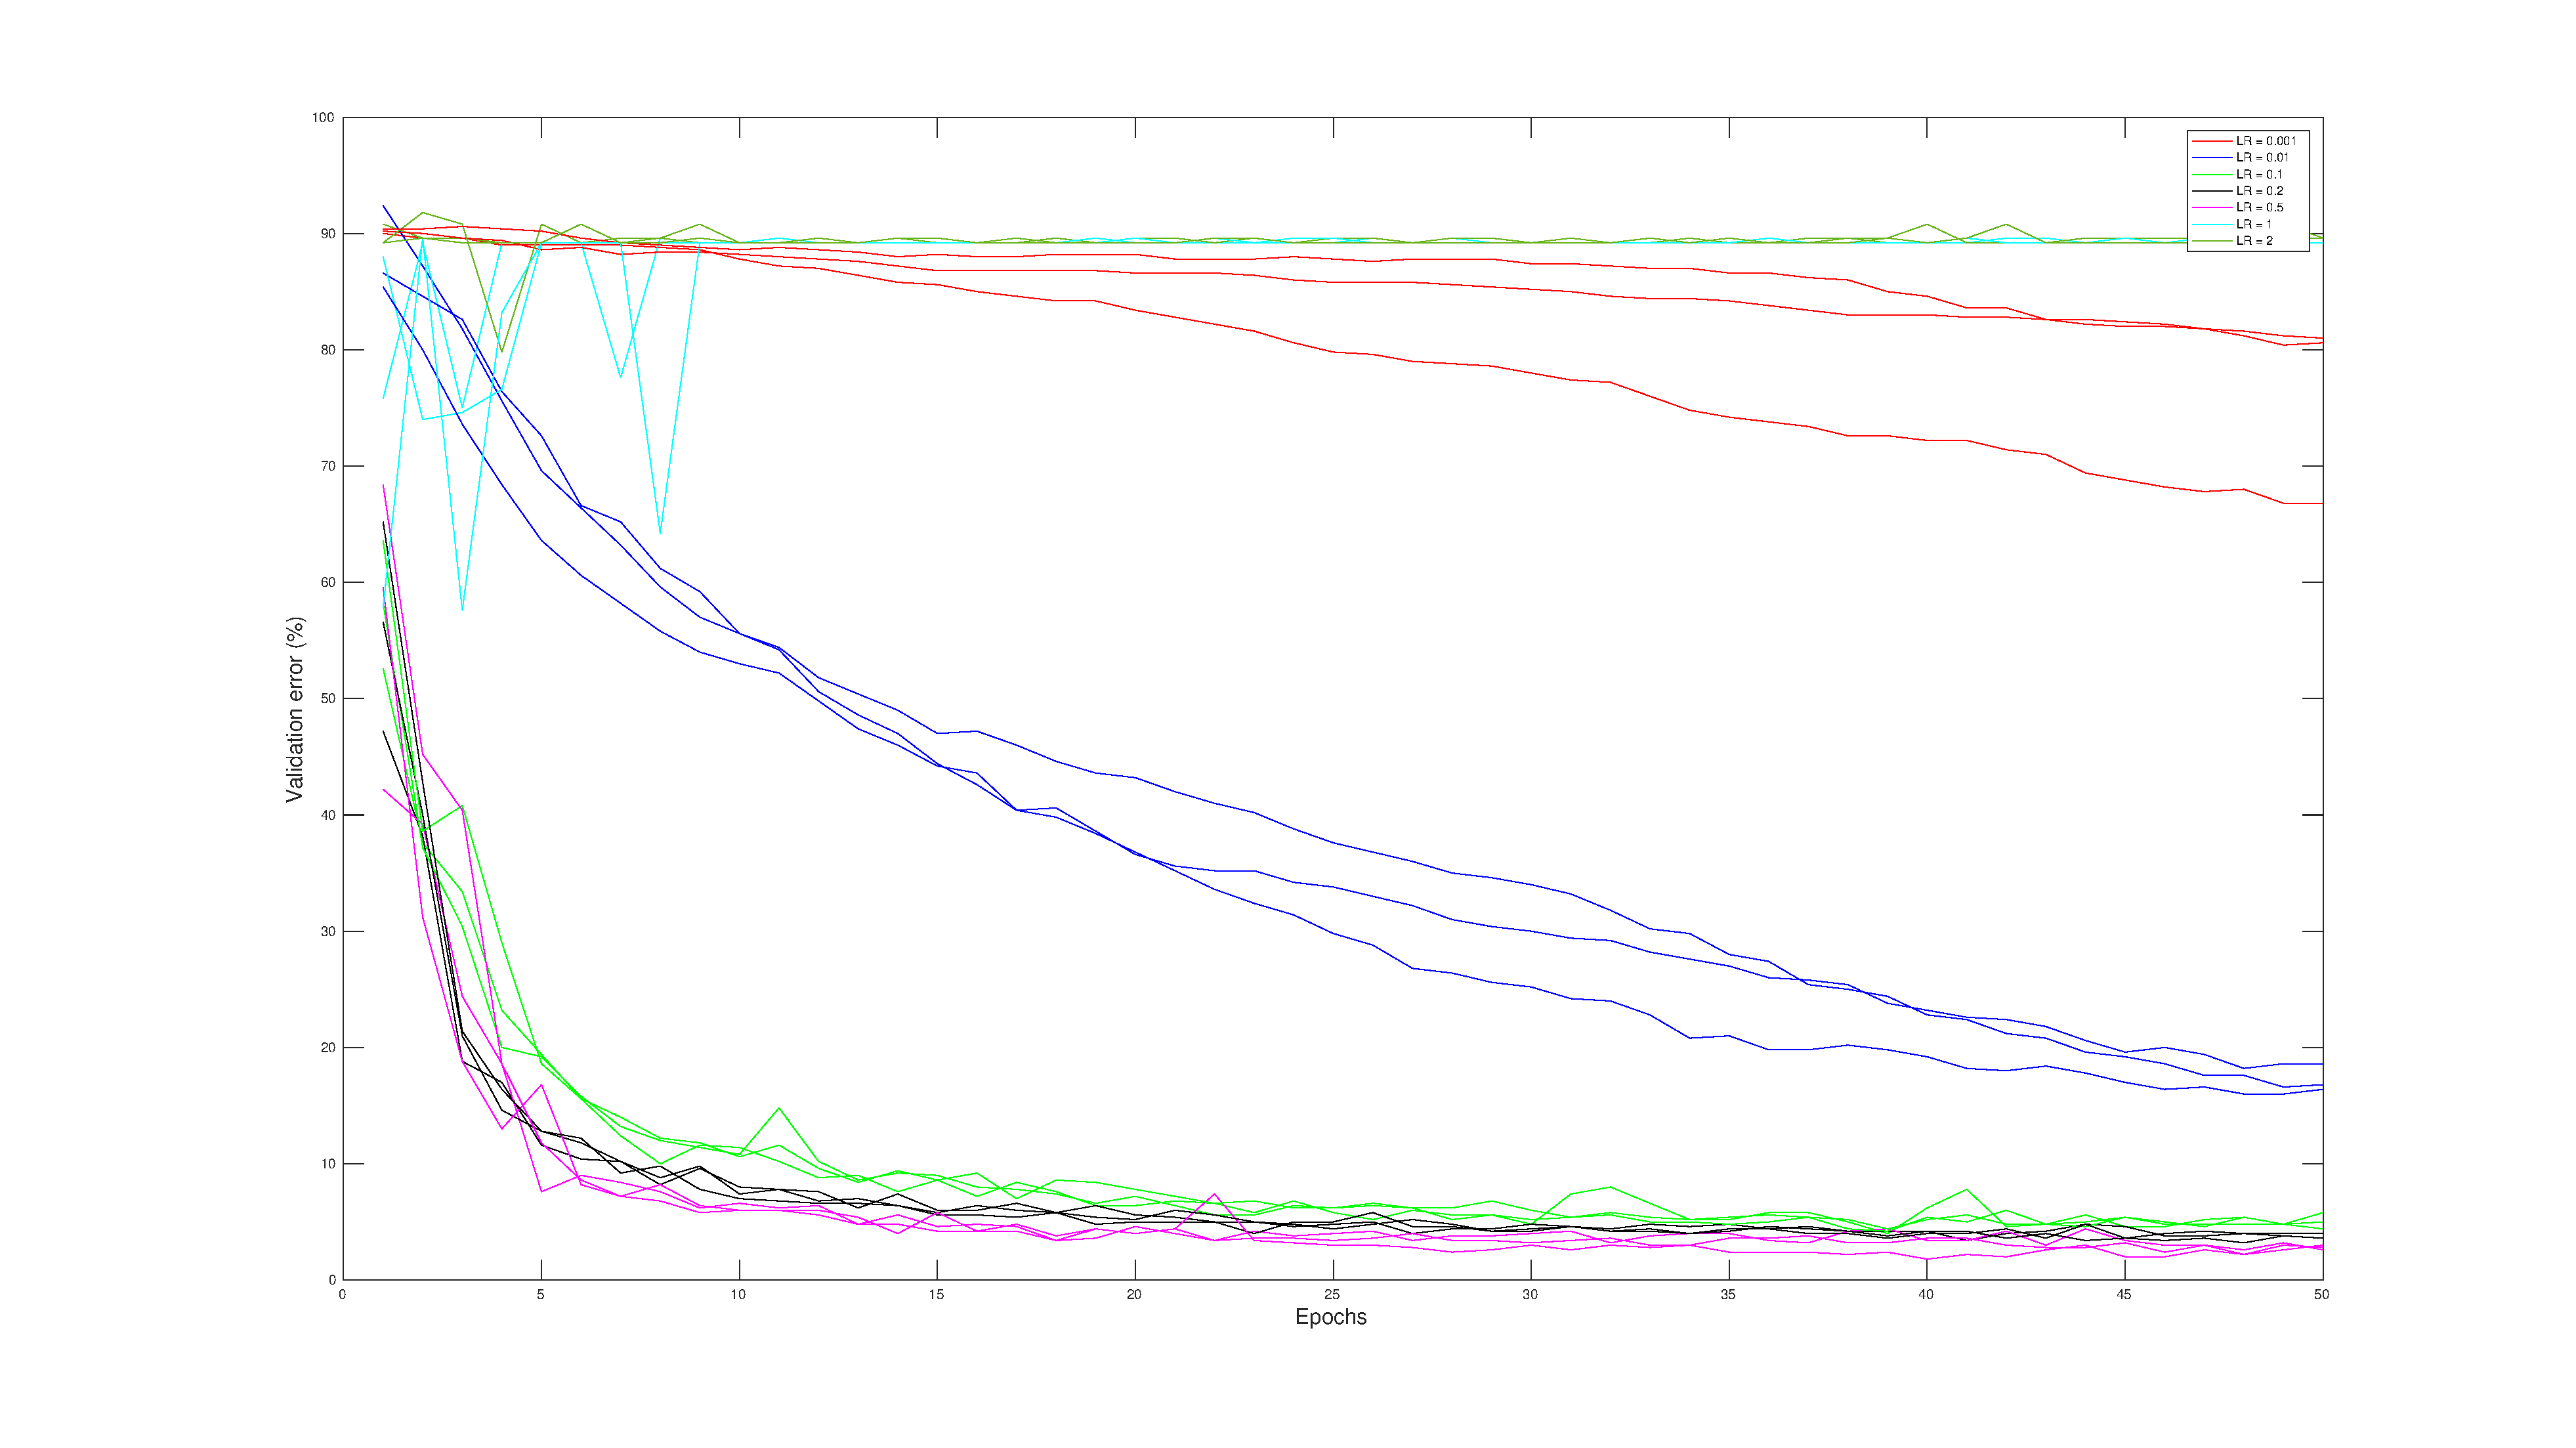
\includegraphics[width=\textwidth]{figures/sc1_val_err}
        \captionsetup{labelformat=empty}
        \caption{Figure 1.3}
    \end{figure}
    
    The learning rate sets the size of the steps taken in gradient descent, so the learning reates that work best are the ones that do steps small enough not to miss the minumum by overshooting it,
    while still providing a reasonably fast and effective descent. 
    
    The overshooting phenomenon can be seen in the plot for the biggest rates $LR = \{1,2\}$: for $LR = 2$ it's immediate, then the network sets to a constant loss 
    not, being able to hit a "valley" to descend.
    For $LR = 0.001$ (too small) the training loss decreases extremely slowly, therefore the network risks to get stuck in suboptimal minima.
    
    \paragraph*{Sources of stochasticity}
        \begin{itemize}
        \item random weight initialization
        \item SGD: randomly selected minibatches
        \item dropouts
        \end{itemize}
    
    
    
    
\section*{Scenario 2}
	\begin{figure}[!htb]
        \centering
        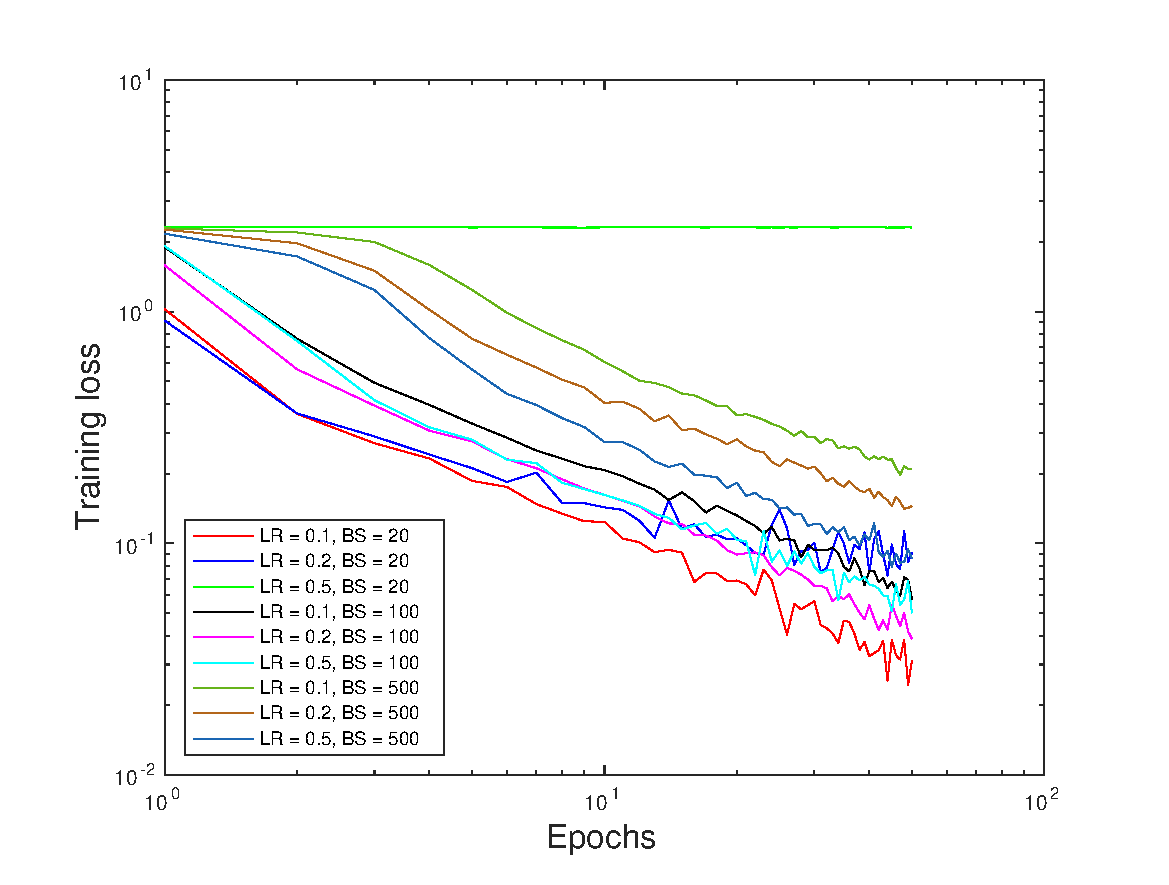
\includegraphics[width=\textwidth]{figures/sc2_tr_loss}
        \captionsetup{labelformat=empty}
        \caption{Figure 2.1}
    \end{figure}
    \begin{figure}[!htb]
        \centering
        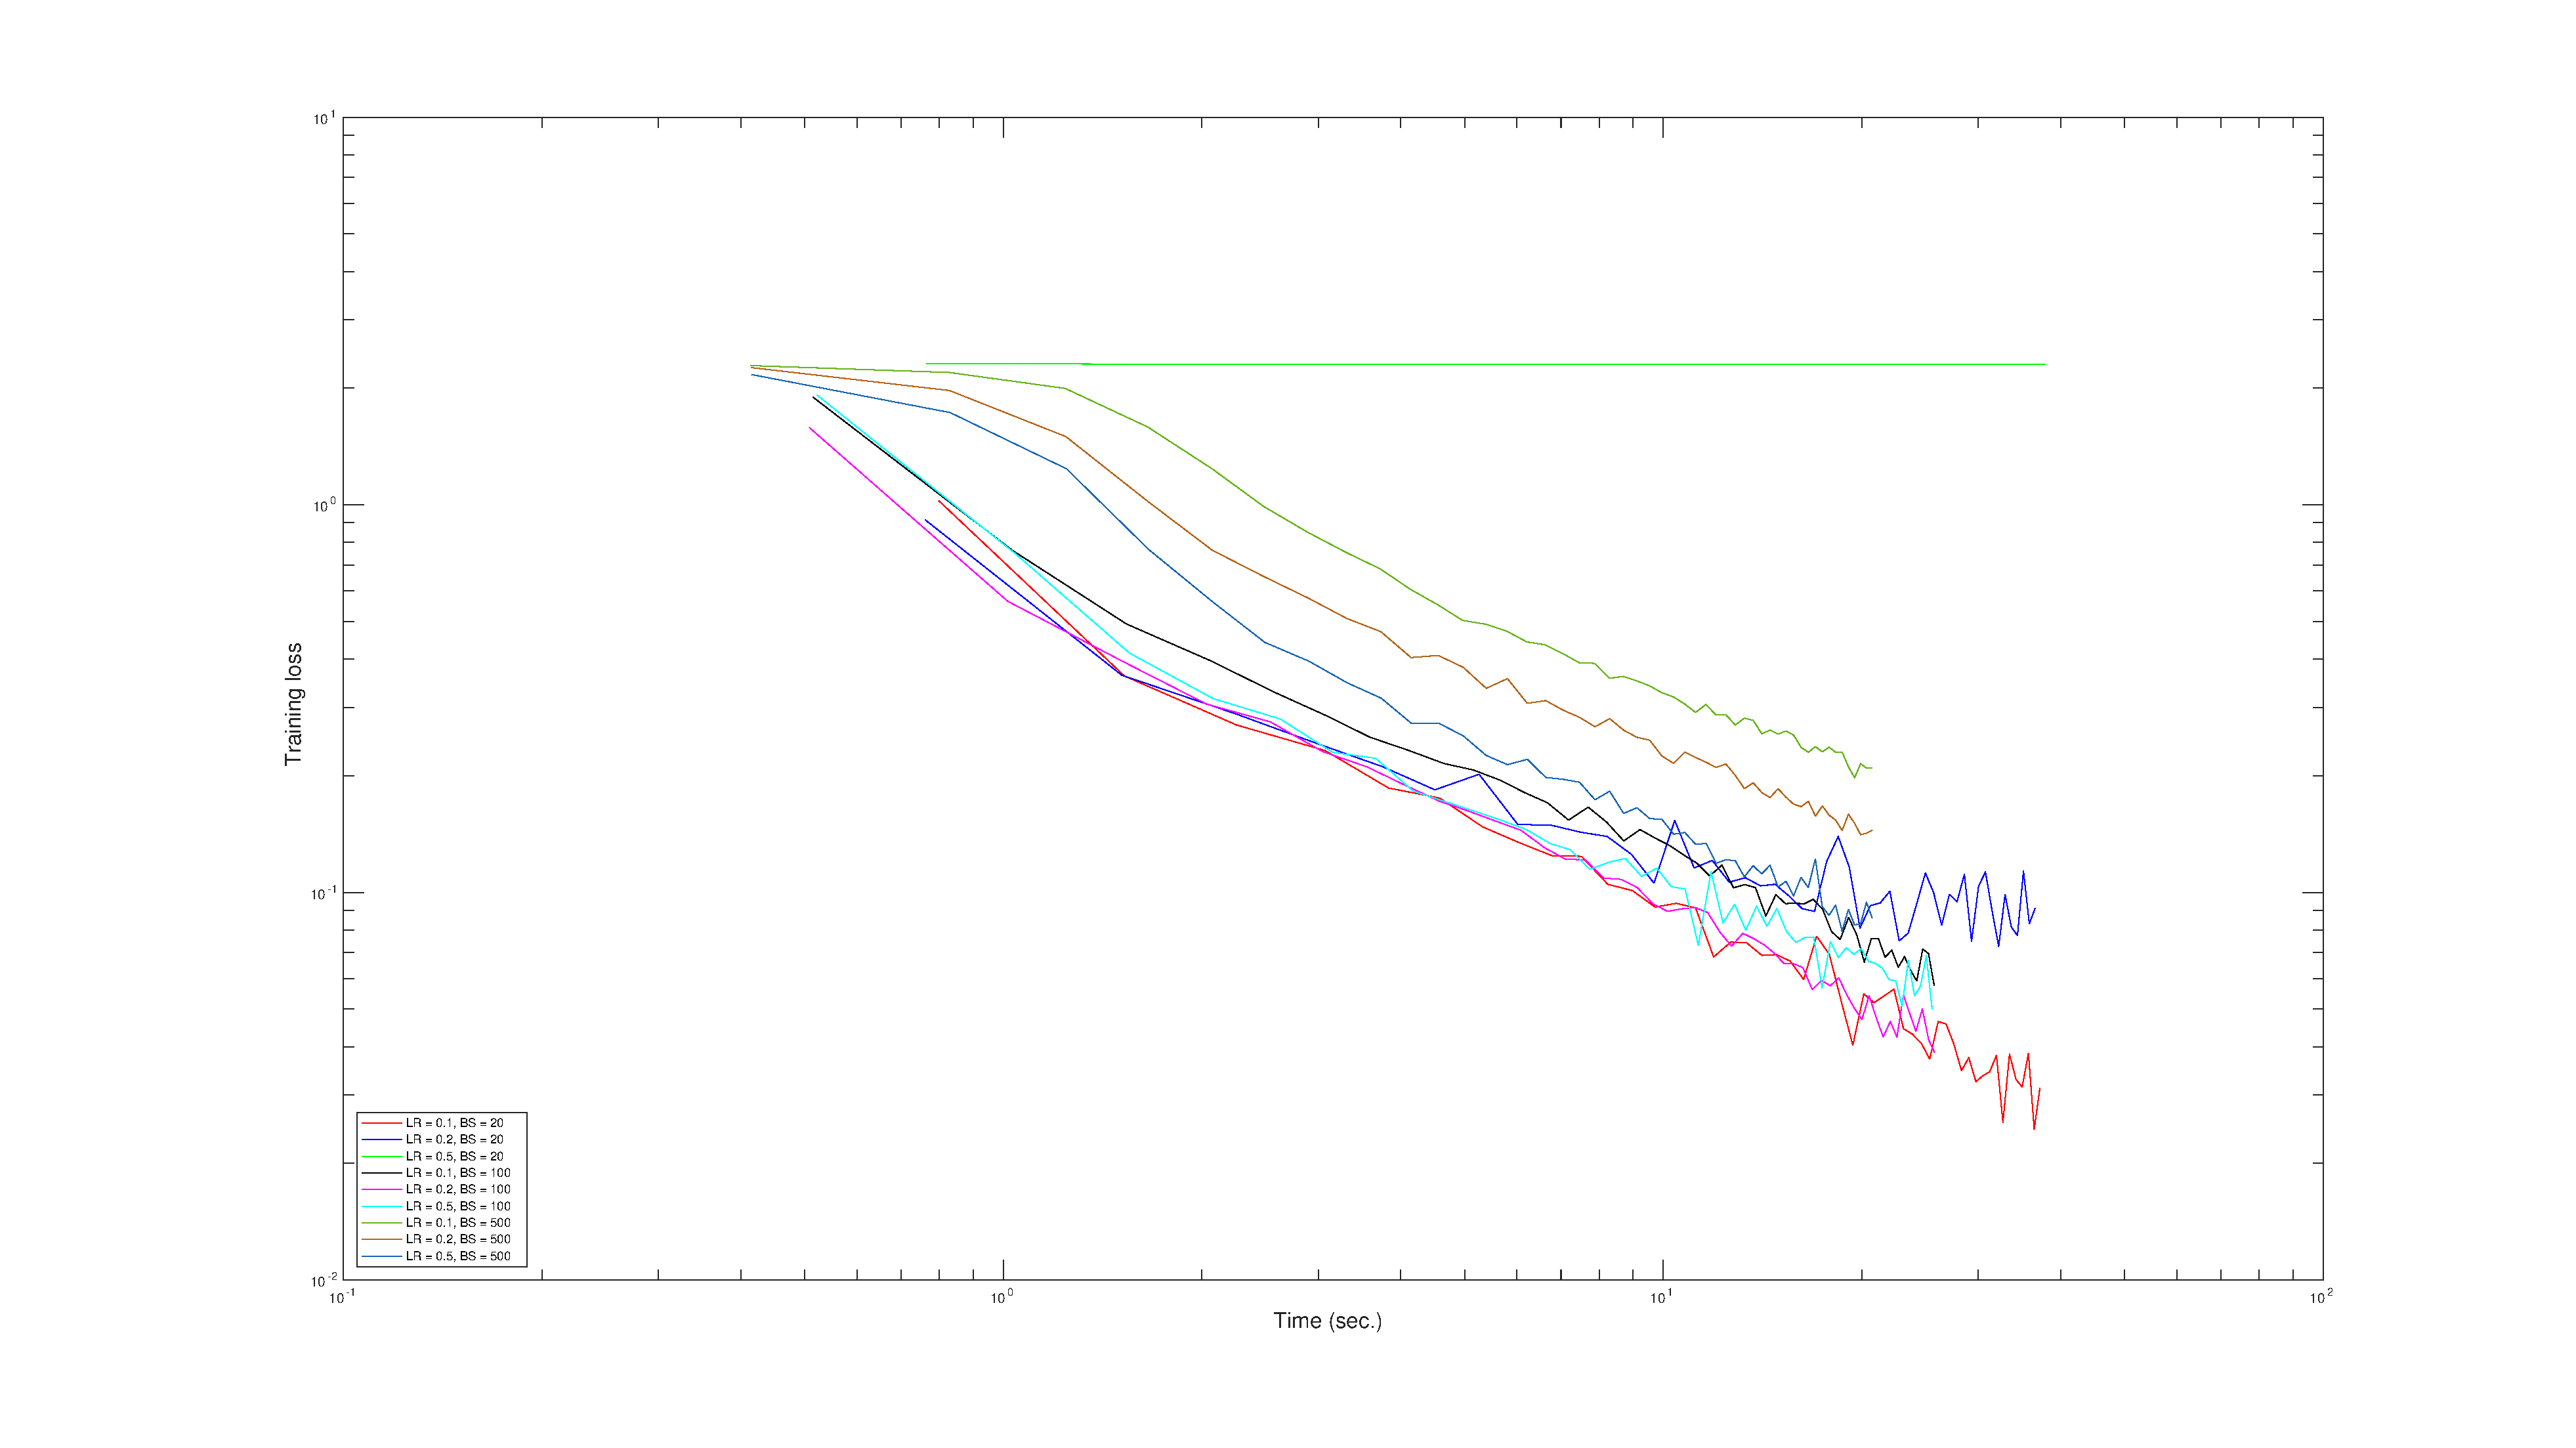
\includegraphics[width=\textwidth]{figures/sc2_tr_loss_time}
        \captionsetup{labelformat=empty}
        \caption{Figure 2.2}
    \end{figure}

    With the smallest batch size of 20, the best rate is $LR = 0.1$, and this configuration also gives the best overall result. With $BS = 100$ the best learning rate is 0.2, and for $BS = 500$ is $LR = 0.5$.
    The best results are therefore obtained with directly proportional hyperparameters.
    
    The smaller the batch size, the less accurate the gradient estimate on which the network trains (higher variance between the estimated loss gradients), so it makes sense to use a smaller learning rate
    and not make overconfident descent steps on noisy gradients. The noisy descent can be already seen in the learning curve of $BS = 20, LR = 0.1$; with $BS = 20, LR = 0.2$ there is a worse descent on average; 
    with $BS = 20, LR = 0.5$ the network is completely unable to perform descent. Larger batch sizes have smoother curves but slower descents, because the network does less steps per epoch.
    
    The setups have different training times, and they are not different by a factor of five, because the operations done on the batches have nonlinear time complexity w.r.t. the batch size.
    
    
    
\section*{Scenario 3}
	\begin{figure}[!htb]
        \centering
        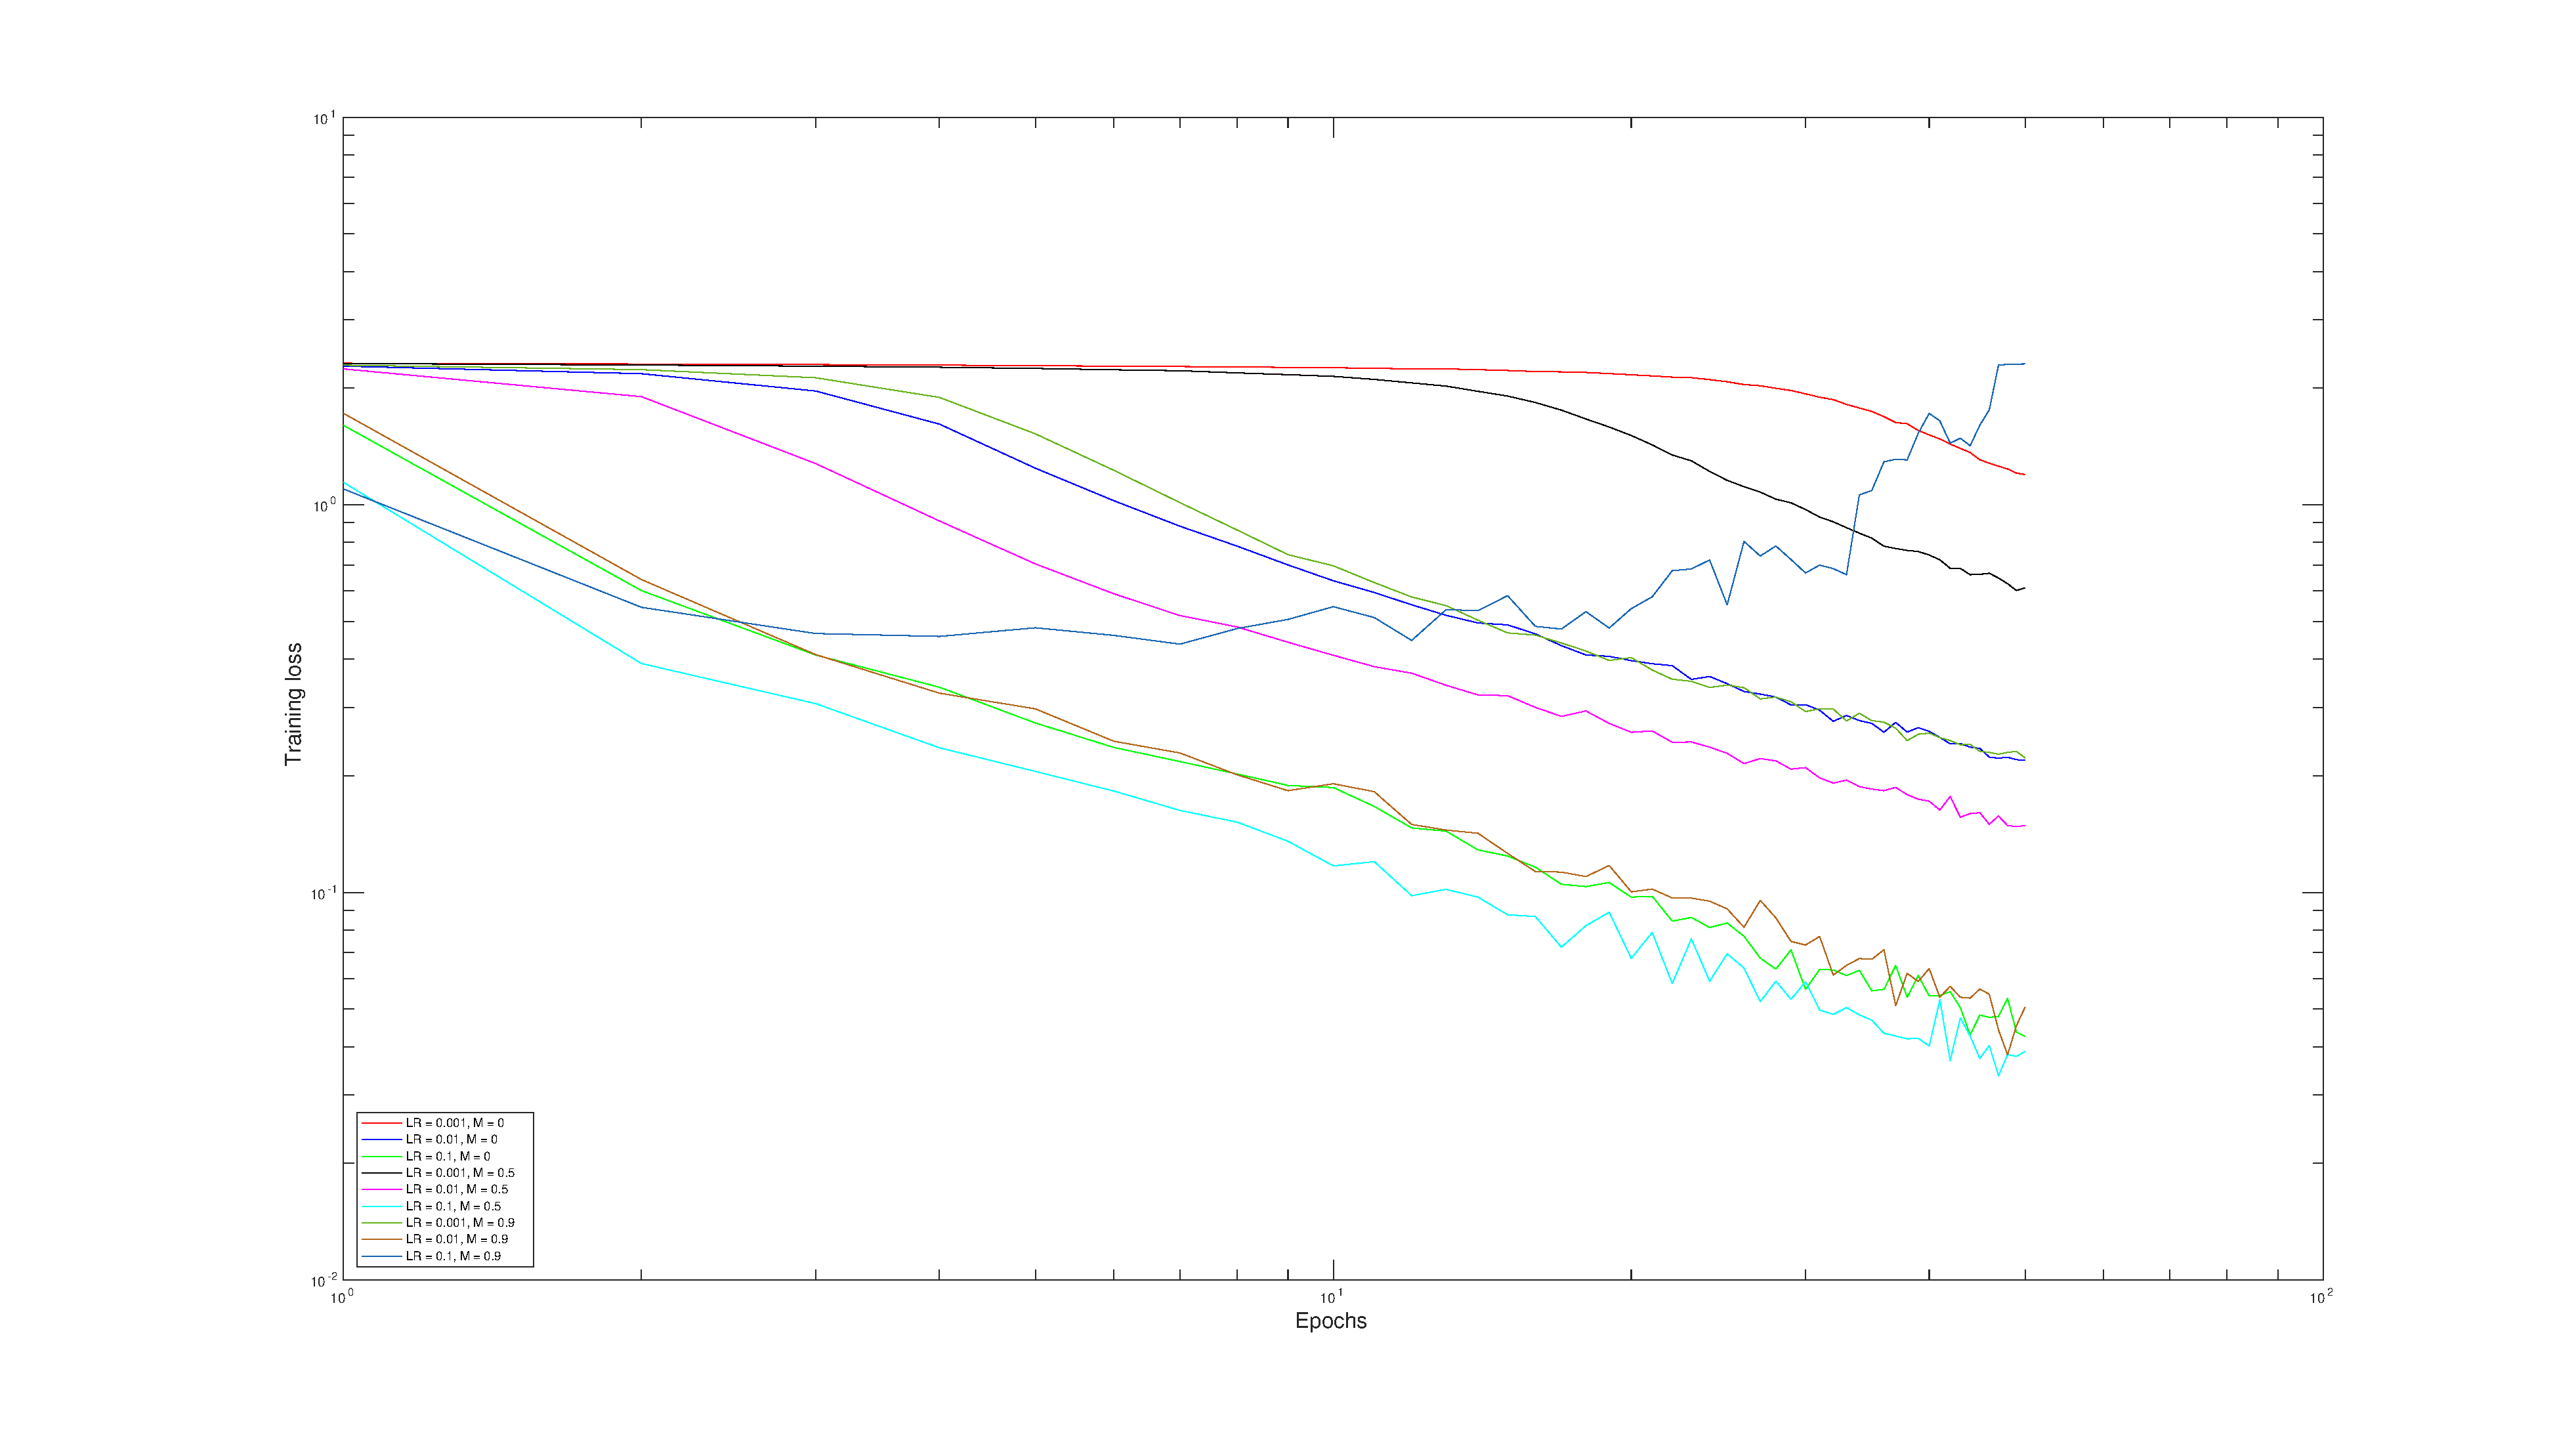
\includegraphics[width=\textwidth]{figures/sc3_tr_loss}
        \captionsetup{labelformat=empty}
        \caption{Figure 3.1}
    \end{figure}
    
    The plots show that a balanced combination between learning rate and momentum works best. The best hyperparameter configurations are, in decreasing order, 
    $LR = 0.1, M = 0.5$, $LR = 0.01, M = 0.9$ and $LR = 0.1, M = 0$, showing that a higher momentum can help smaller learning rates to get a better performance. 
    
    This is evident watching the red, black, and dark green curves, which are relative to the smallest learning rate (0.001): with this rate the network still learns very slowly, but we can see the positive effect of the momentum. 
    This effect is to help the descent algorithm to overcome local minima and to speed up the training accumulating velocity when possible.
    
    The only case where a big momentum is counterproductive is with $LR = 0.1$: in this case the combination between (relatively) high $LR$ and high momentum make the network diverge by "climbing" uphill the loss function.
    
    
    
    
\section*{Scenario 4}
	\begin{figure}[!htb]
        \centering
        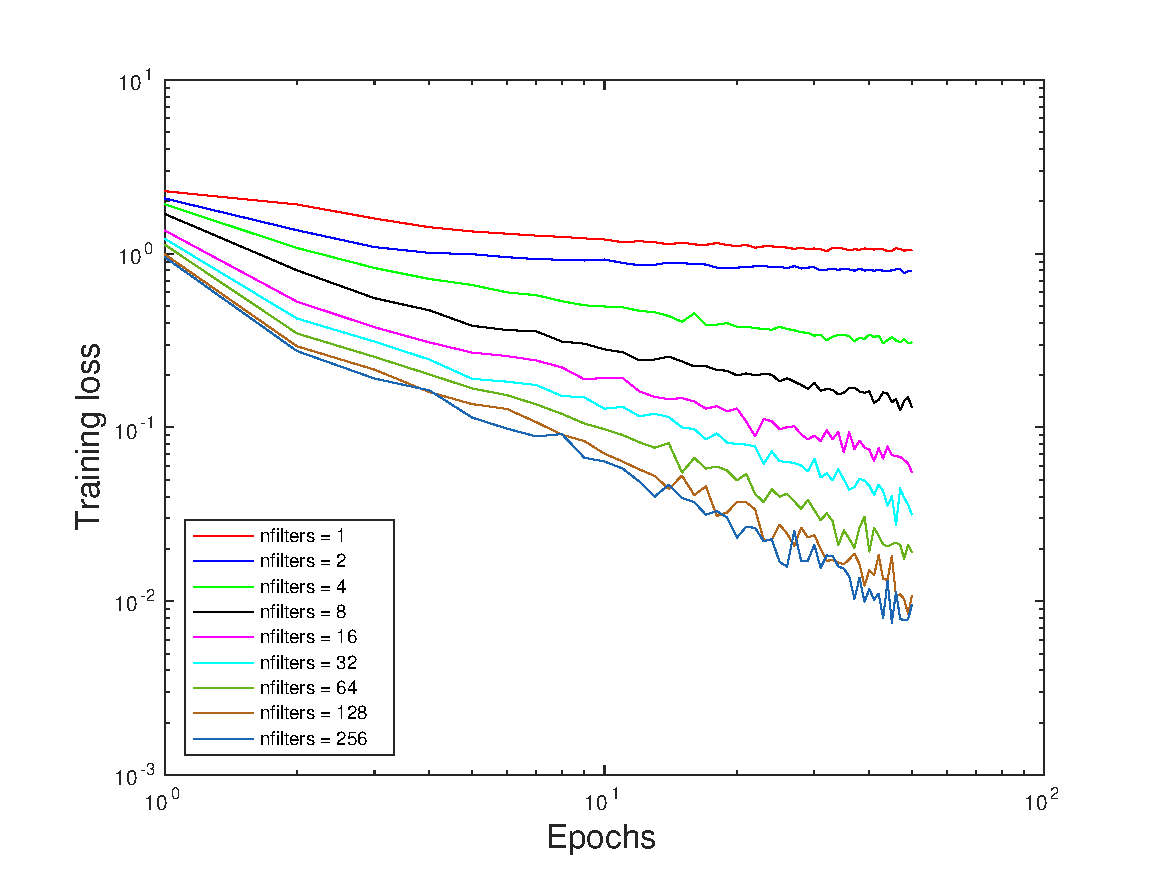
\includegraphics[width=\textwidth]{figures/sc4_tr_loss}
        \captionsetup{labelformat=empty}
        \caption{Figure 4.1}
    \end{figure}
    \begin{figure}[!htb]
        \centering
        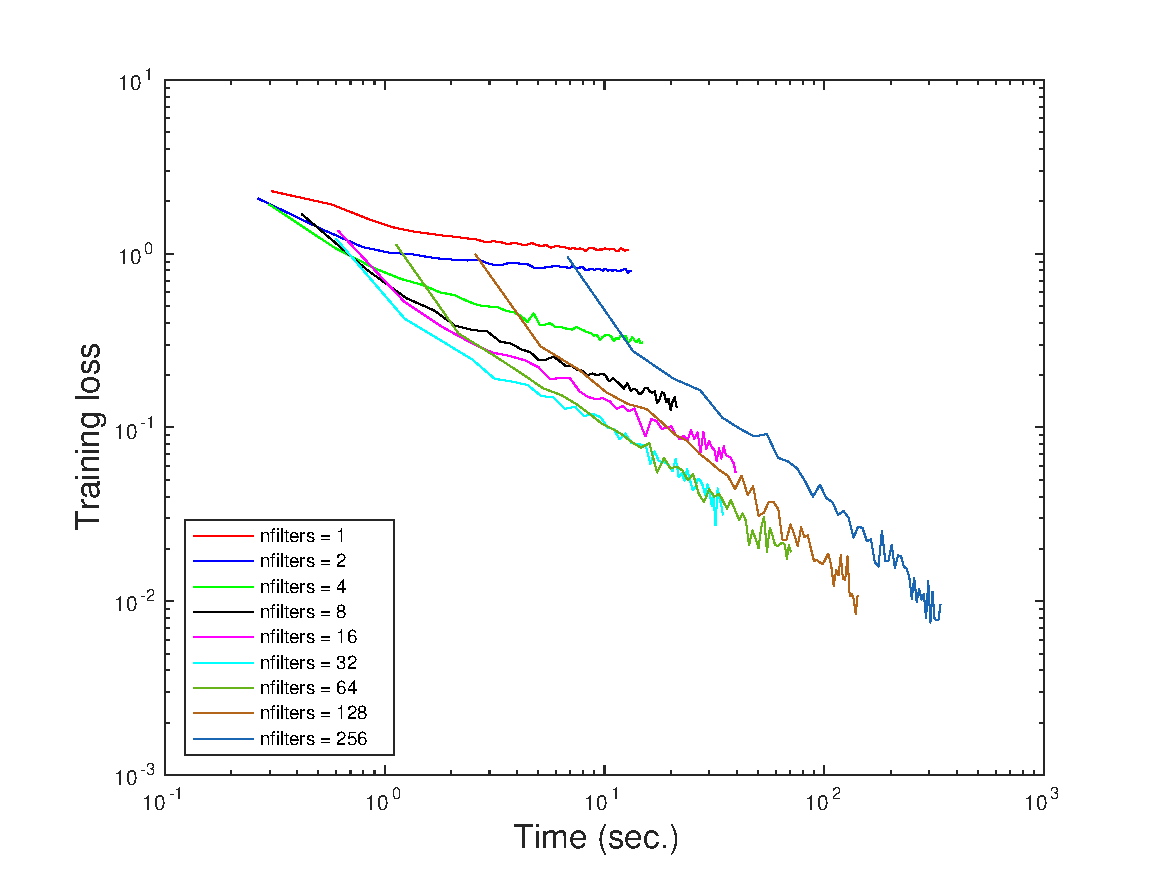
\includegraphics[width=\textwidth]{figures/sc4_tr_loss_time}
        \captionsetup{labelformat=empty}
        \caption{Figure 4.2}
    \end{figure}
    \begin{figure}[!htb]
        \centering
        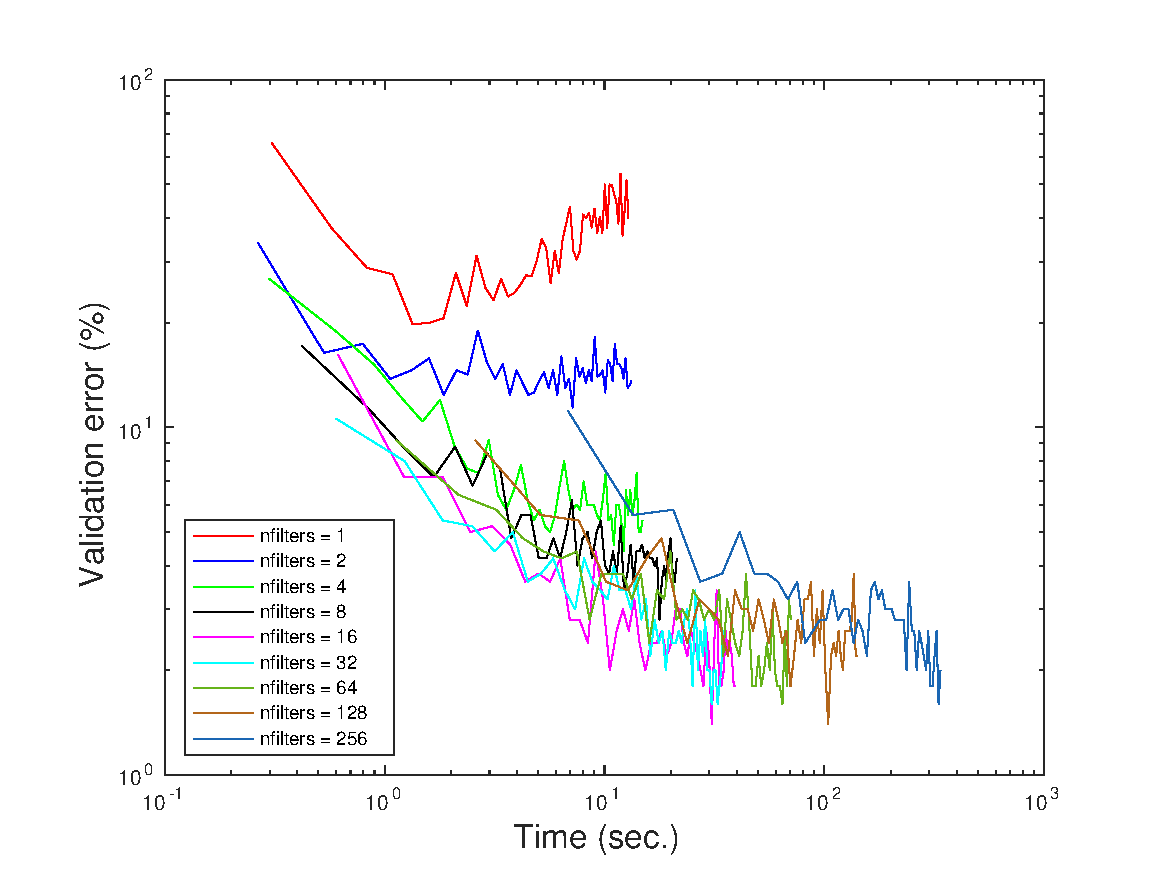
\includegraphics[width=\textwidth]{figures/sc4_val_err_time}
        \captionsetup{labelformat=empty}
        \caption{Figure 4.3}
    \end{figure}
    
    In the first plot the final training loss is inversely proportional to the number of filters used: with 1-2 layers the network performs badly,
    increasing nfilters it gets better, until the top performance of 128-256 filters. With many filters, however, the training error curves become
    progressively "noisier". 
    
    This is possibly caused by the fact that many parameters make the gradient estimate less accurate;
    another hypothesis is that the network is not fitting on the common features anymore, 
    but instead on more example-specific details or noise.
    However, it would be better to choose some intermediate and more stable number of filters, like 32.
    
    The plot of training loss over time shows how longer it takes for a network with many filters to achieve the same loss of simpler ones, 
    independently from the number of epochs. 
    In 10 seconds the best performing networks have 32 and 64 filters, so this would be chosen with such a time limitation.
    
    The third plot confirms that it would be better to choose a number of filters like 16 or 32, as they are the best performing in terms of time and error.
    The plot also suggests that it would make sense to choose a smaller learning rate and/or a bigger batch size, to reduce the oscillation of the learning curves.
    
    
    
\section*{Scenario 5}
    
    \begin{figure}[!htb]
        \centering
        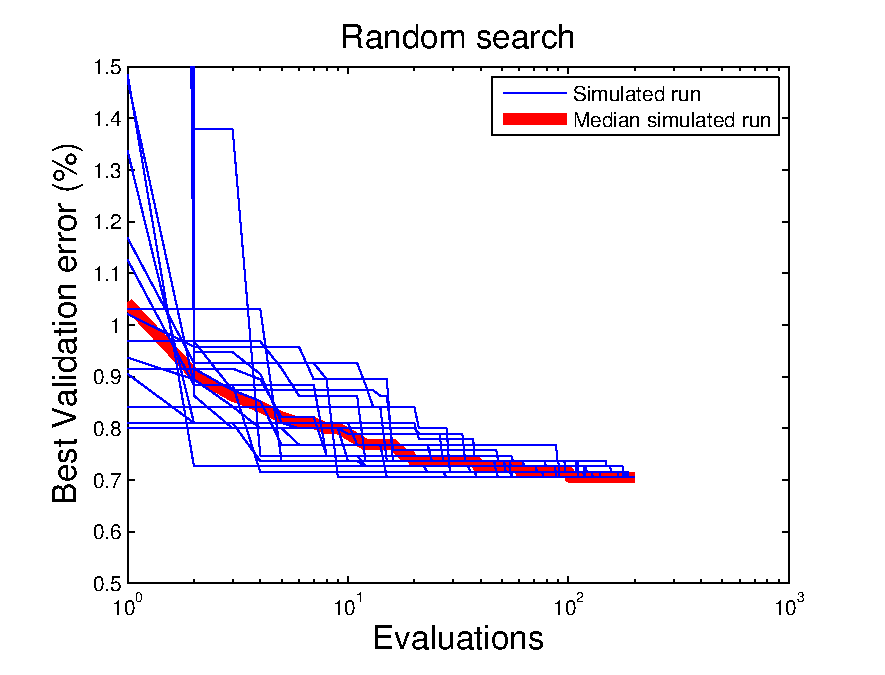
\includegraphics[width=\textwidth]{figures/sc5}
        \captionsetup{labelformat=empty}
        \caption{Figure 5.1}
    \end{figure}
    
    \paragraph{Best configurations}
        The best results (validation accuracy $> 99.20\%$) for a run of the 5th scenario were:
        \vspace{10px}\\
        nfilters = 55, BS = 94, M = 0.53, LR = 0.09: validation accuracy = 99.32\% \\
        nfilters = 29, BS = 22, M = 0.19, LR = 0.09: validation accuracy = 99.27\% \\
        nfilters = 27, BS = 28,	M = 0.51, LR = 0.08: validation accuracy = 99.24\% \\
        nfilters = 27, BS = 157, M = 0.68, LR = 0.13: validation accuracy = 99.21\% \\
        nfilters = 36, BS = 104, M = 0.54, LR = 0.24: validation accuracy = 99.21\% \\
        
        It can be seen that these configurations are similar to the best ones found in the previous scenarios.
        The number of filters is bounded in a range between 27 and 47, the batch size between 22 and 157, and
        the learning rate is neither much lower than 0.1 nor higher than 0.3. The momentum varies a bit more, 
        but in scenario 3 the best learning rate - momentum combination was $LR \approx 0.1, M \approx 0.5$, and this is still the case here, 
        with some variation depending on the other parameters.
    
    
\section{Scenario 6}
    The communication works with the scripts \texttt{master.py} and \texttt{worker.py}. The latter relies on the script \texttt{exercise3.py} to evaluate the hyperparameter settings, and thus requires it to be in the same folder.
    First we run the master script, which stores the settings in logfiles placed in the \texttt{logs/} folder, then - with master still running - we can launch different workers from different machines.
    The workers will read the log files and train the network based on the given settings, and once finished they will write the obtained performance on the same files. 
    To keep track of the status of the log files, the scripts append them file extensions (\texttt{.taken}, \texttt{.done}, \texttt{.seen}). This makes the filenames look a bit silly, but it works.
    
\end{document}
